\section{Resultados}

En esta sección se presentarán los resultados iniciales obtenidos de un primer modelo con 100k de datos de entrenamiento y un segundo modelo con 500k de datos de entrenamiento. Se presentarán las curvas de pérdida y precisión de los modelos así como las curvas de precisión top-k. Además de eso, veremos más adelante los resultados de la policy head de los modelos, que nos permitirán ver si el modelo es capaz de aprender a predecir la probabilidad de cada tile de ser descartado en un estado de juego dado.

Para cada modelo, se presentarán las curvas de pérdida y de precisión top-1 de testeo y validación, luego se presentarán en conjunto las curvas top-3 y top-5 de validación. A continuación se presentará la distribución de confianza del modelo y finalmente los resultados de la precisión cuando separadas por categorías semánticas de error basadas en el Shanten \ref{seubsec:shanten} y el Ukeire \ref{seubsec:ukeire} que será presentado en una sección posterior de comparación de modelos.



\subsection{Primer Modelo}

Este primer modelo fue entrenado con 100k de datos de entrenamiento, 10k de validación y 10k de testeo. El modelo fue entrenado durante 15 épocas, con un batch size de 64 y un learning rate de 1e-4. A continuación se presentan las curvas de pérdida y precisión del modelo durante el entrenamiento y la validación.

\begin{figure}[H]
    \centering
    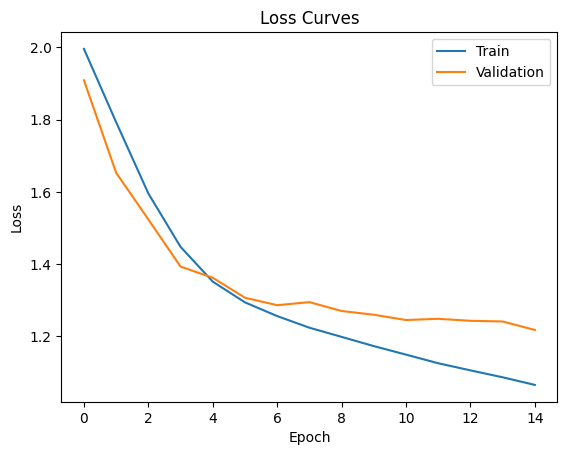
\includegraphics[width=0.8\textwidth]{figures/01_loss_curves.png}
    \caption{Curvas de pérdida y precisión del primer modelo con 100k de datos de entrenamiento.}
    \label{fig:loss_curves_100k}
\end{figure}
  
\begin{figure}[H]
    \centering
    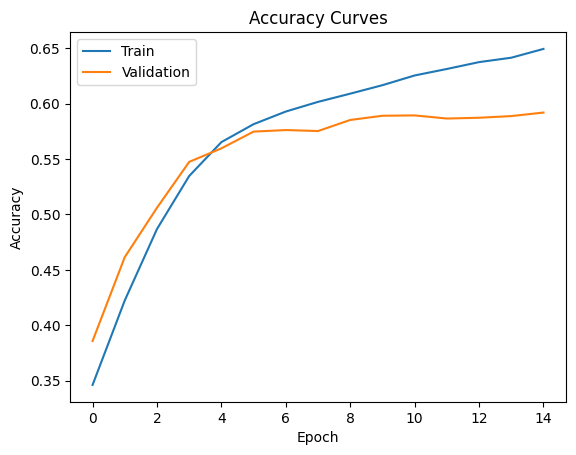
\includegraphics[width=0.8\textwidth]{figures/01_accuracy_curves.png}
    \caption{Curvas de pérdida y precisión del primer modelo con 100k de datos de entrenamiento.}
    \label{fig:accuracy_curves_100k}
\end{figure}

\begin{figure}[H]
    \centering
    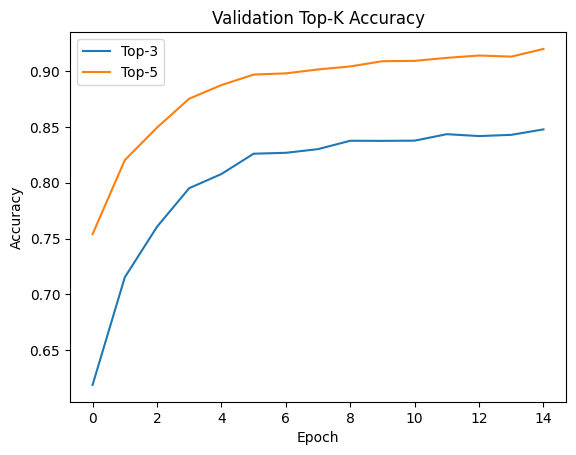
\includegraphics[width=0.8\textwidth]{figures/01_top_k_accuracy.png}
    \caption{Curvas de precisión top-k del primer modelo con 100k de datos de entrenamiento.}
    \label{fig:top_k_accuracy_100k}
\end{figure}
    
Con estos resultados obtuvimos un serie de observaciones importantes: la primera es que el modelo no llegó a la saturación de la precisión, lo que nos indica que el modelo no está sobreajustando los datos de entrenamiento y que podría mejorar con más datos de entrenamiento. La segunda observación es que apesar de que la precisión top-1 del modelo es de 0.65 para los datos de entrenamiento y 0.591 para los datos de valisación, la precisión top-3 es de 0.84 y la top-5 es de 0.91, lo que indica que el modelo es capaz de aprender a predecir los descartes de Mahjong a partir del diseño y la arquitectura que tenemos, y que con más datos de entrenamiento podría mejorar su precisión top-1.

A seguir podemos ver el gráfico de distribución de confianza del modelo, que nos permite ver la distribución de la probabilidad de los descartes predichos por el modelo.

\begin{figure}[H]
    \centering
    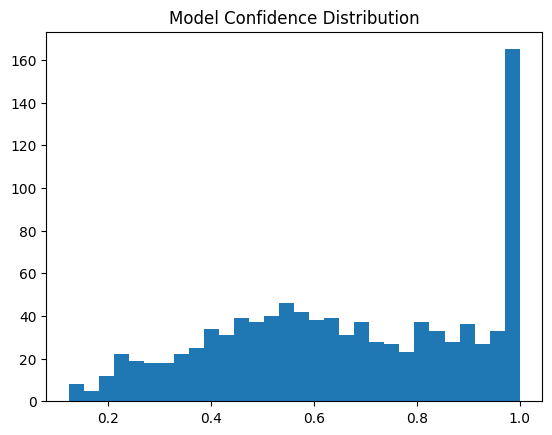
\includegraphics[width=0.8\textwidth]{figures/01_model_confidence.png}
    \caption{Distribución de confianza del primer modelo con 100k de datos de entrenamiento.}
    \label{fig:confidence_distribution_100k}
\end{figure}

Con este gráfico podemos ver que el modelo tiene un pico en la probabilidad de 1.0. Este pico indica una confianza del 100\% en muchas de las predicciones del modelo, no obstante, esta confianza puede ser explicada con los estados de juego en el que existe una única opción de descarte. Para arreglar esto, se realizó una limpieza de datos para eliminar los estados de juego en los que existe una única opción de descarte para el entrenamiento del próximo modelo, que será presentado a continuación.

\subsection{Segundo Modelo}

Este segundo modelo fue entrenado con 500k de datos de entrenamiento, 50k de validación y 50k de testeo. El modelo fue entrenado durante 15 épocas, con un batch size de 64 y un learning rate de 1e-4. A continuación se presentan las curvas de pérdida y precisión del modelo durante el entrenamiento de las épocas 9 a 15. El dataset de entrenamiento también fue limpiado para eliminar los estados de juego en los que existe una única opción de descarte.

\begin{figure}[H]
    \centering
    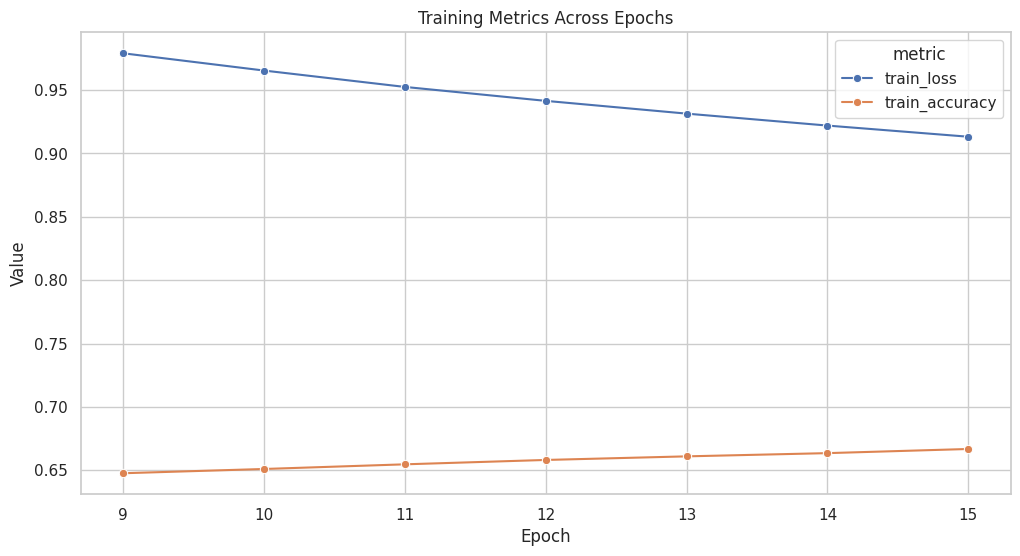
\includegraphics[width=0.8\textwidth]{figures/02_training_metrics.png}
    \caption{Curvas de pérdida y precisión del segundo modelo con 500k de datos de entrenamiento.}
    \label{fig:loss_curves_500k}
\end{figure}
    
Y en esta figura podemos ver el gráfico de distribución de confianza del modelo ajustado sin los estados de juego en los que existe una única opción de descarte.

\begin{figure}[H]
    \centering
    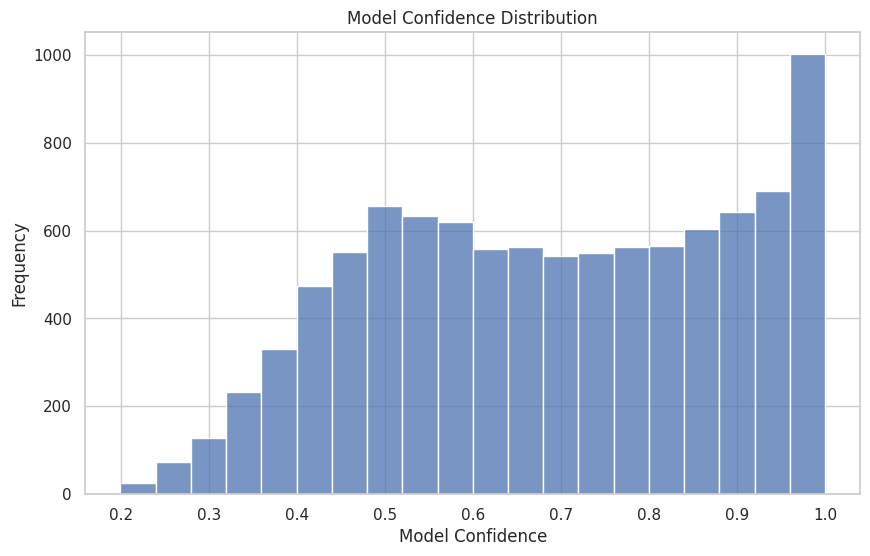
\includegraphics[width=0.8\textwidth]{figures/02_model_confidence.png}
    \caption{Distribución de confianza del segundo modelo con 500k de datos de entrenamiento.}
    \label{fig:confidence_distribution_500k}
\end{figure}

Podemos ver que pese a la disminución de la confianza del modelo, el modelo sigue teniendo un pico en la probabilidad de 1.0, lo que indica que el modelo sigue teniendo una confianza del 100\% en muchas de sus predicciones. Además de eso, podemos ver que la tiene un segundo pico en el 0.5 donde se mantiene estable hasta el 0.9. Estos resultados indican una buena confianza del modelo en sus predicciones, principalmente si consideramos que en su mayoria de los estados de juego existen 13 opciones de descarte posibles en media.

\subsection{Validación Estratégica}

La validación estratégica es un proceso que nos permite evaluar la capacidad del modelo para predecir descartes de Mahjong en función de la estrategia de juego. Para ello, se utilizaron métricas basadas en el Shanten y el Ukeire, que nos permiten clasificar los errores del modelo en diferentes categorías semánticas.

Las categorias creadas son las siguientes:

\begin{itemize}
    \item Exact match: el descarte predicho por el modelo coincide exactamente con el descarte real del jugador.
    \item Equivalent: el descarte predicho por el modelo resulta en el mismo Shanten y Ukeire que el descarte real del jugador.
    \item Better shanten: el descarte predicho por el modelo resulta en un Shanten menor que el descarte real del jugador.
    \item Better ukeire: el descarte predicho por el modelo resulta en un Ukeire mayor que el descarte real del jugador.
    \item Near equivalent: el descarte predicho por el modelo resulta en un Shanten y Ukeire que difieren en máximo dos unidades del descarte real del jugador.
    \item Shanten loss: el descarte predicho por el modelo resulta en un Shanten mayor que el descarte real del jugador.
    \item Ukeire loss: el descarte predicho por el modelo resulta en un Ukeire menor.
\end{itemize}

\subsubsection{Validación Estratégica del Primer Modelo}


A partir de 10k de datos de validación, de los cuales todos tienen por lo menos más de una opción de acción válida, se realizó la categorización de cada decisión tomada por la máquina utilizando las categorías mencionadas anteriormente.

En este primer gráfico podemos observar que muchas decisiones buenas, como \textit{better\_shanten} o \textit{better\_ukeire} no fueron llevadas en consideración al \textit{accuracy} del modelo:

\begin{figure}[H]
    \centering
    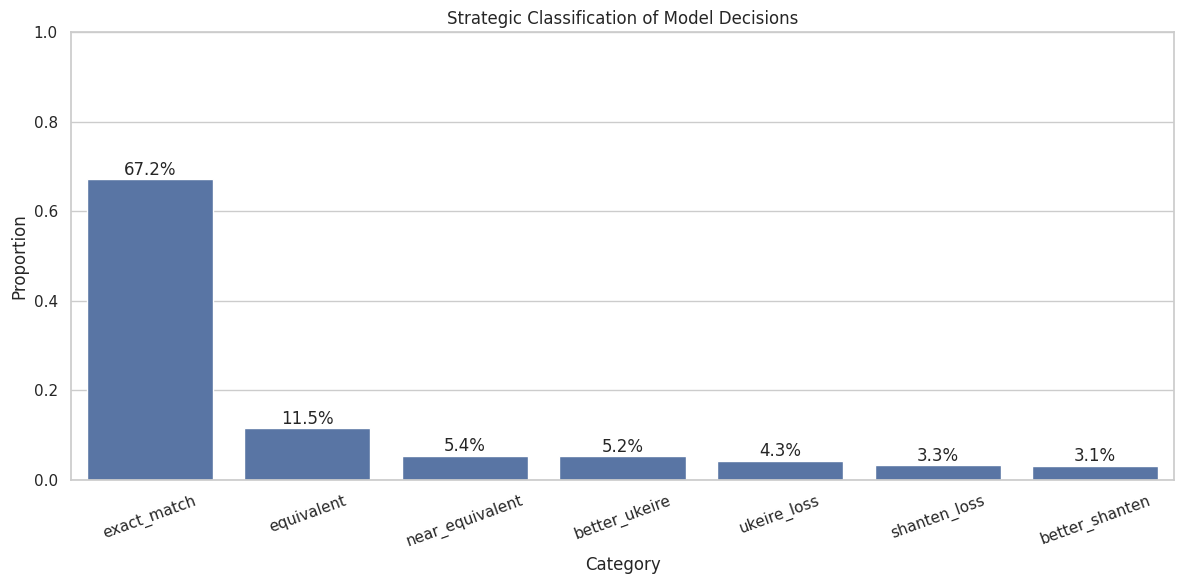
\includegraphics[width=0.8\textwidth]{figures/01_classificacion_estrategica.png}
    \caption{Porcentaje de Cada Categoría Estratégica en el Primer Modelo}
    \label{fig:strategic_class_100k}
\end{figure}

A partir de esto, podemos sacar un valor de \textit{strategic accuracy} mucho mejor que el \textit{accuracy} original, sumando las categorias de \textit{exact\_match, equivalent, better\_ukeire, better\_shanten} obtenemos que el modelo en realidad obtuvo una \textit{accuracy} de 92.4\%.

\begin{figure}[H]
    \centering
    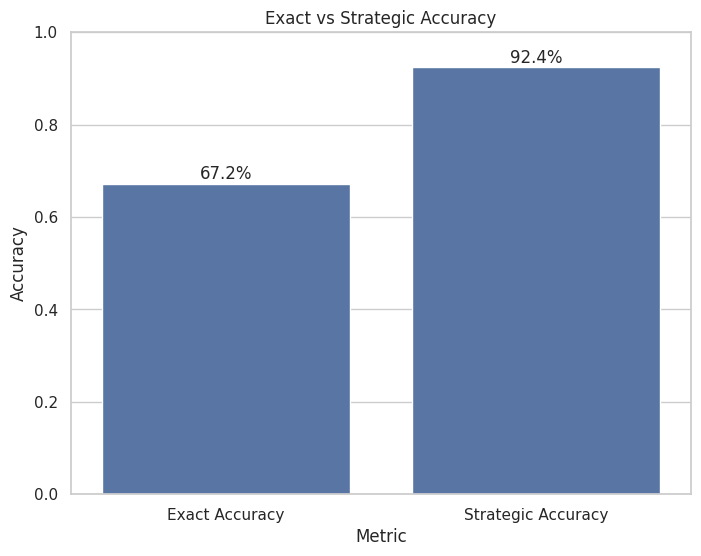
\includegraphics[width=0.8\textwidth]{figures/01_exactvstrategic.png}
    \caption{Comparación validación de accuracy exacta vs accuracy estratégica en el Primer Modelo}
    \label{fig:exact_vs_strat_100k}
\end{figure}

En esta figura también podemos ver la confianza dedl modelo sobre estos datos sin la interferencia de la confianza para datos de validación con una sola acción válida:

\begin{figure}[H]
    \centering
    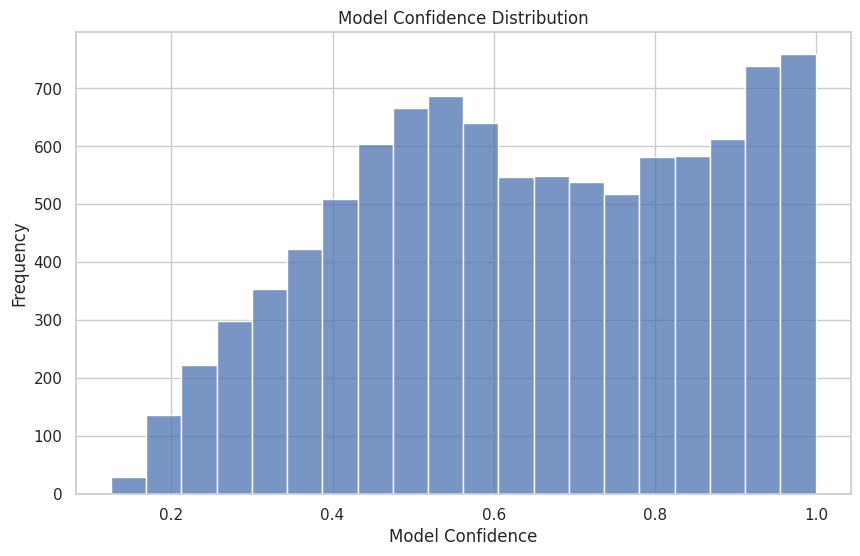
\includegraphics[width=0.8\textwidth]{figures/01_conf_dist_strat.png}
    \caption{Distribución de confianza del primer modelo con ajustado al dataset sin opciones unitárias}
    \label{fig:confidence_distribution_better_100k}
\end{figure}

Como podemos ver, la confianza del modelo está en rangos apropriados para el número de opciones que tiene normalmente (una media de 13 opciones).

Por último, podemos ver también la distribución de confianza del modelo por categoría estretégica, y se percibe que para los casos en que hubo errores graves la confianza del modelo es muy baja en comparación a la confianza en casos de exactitud del modelo, esto indica un buen aprendizaje del modelo.

\begin{figure}[H]
    \centering
    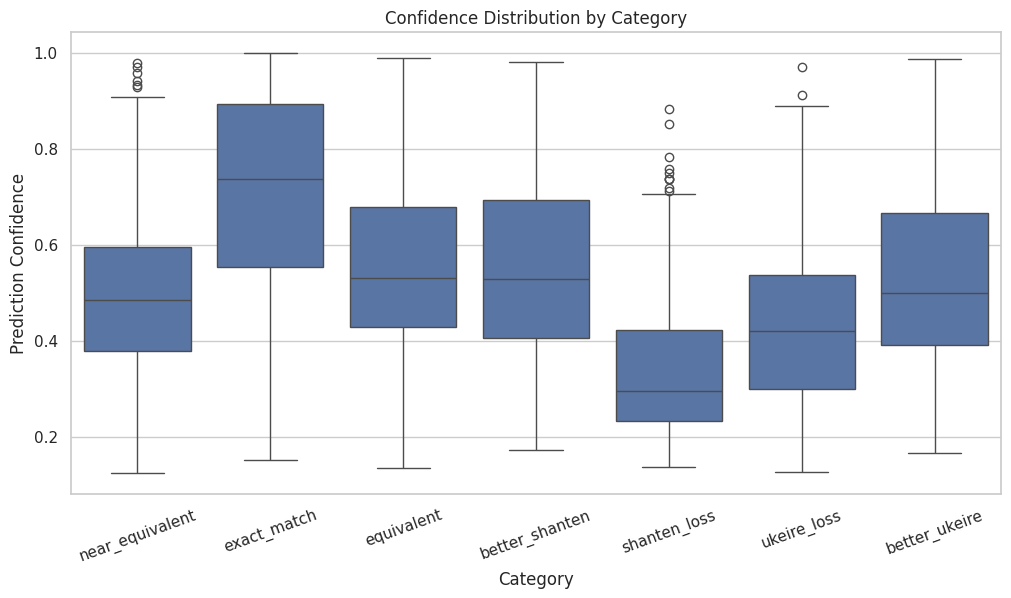
\includegraphics[width=0.8\textwidth]{figures/01_conf_dist_by_cat.png}
    \caption{Distribución de confianza del primer modelo por categoría de la validación estratégica}
    \label{fig:confidence_distribution_by_cat_100k}
\end{figure}

\subsubsection{Validación Estratégica del Segundo Modelo}
De manera análoga al análisis previo, se evaluaron 10k muestras de validación con múltiples opciones de acción válidas para el segundo modelo, aplicando la misma metodología de categorización estratégica.
Al inspeccionar la distribución de las decisiones, observamos cómo el aumento de datos impactan en la consideración de jugadas estratégicamente superiores como \textit{better\_shanten} o \textit{better\_ukeire}:
\begin{figure}[H]
\centering
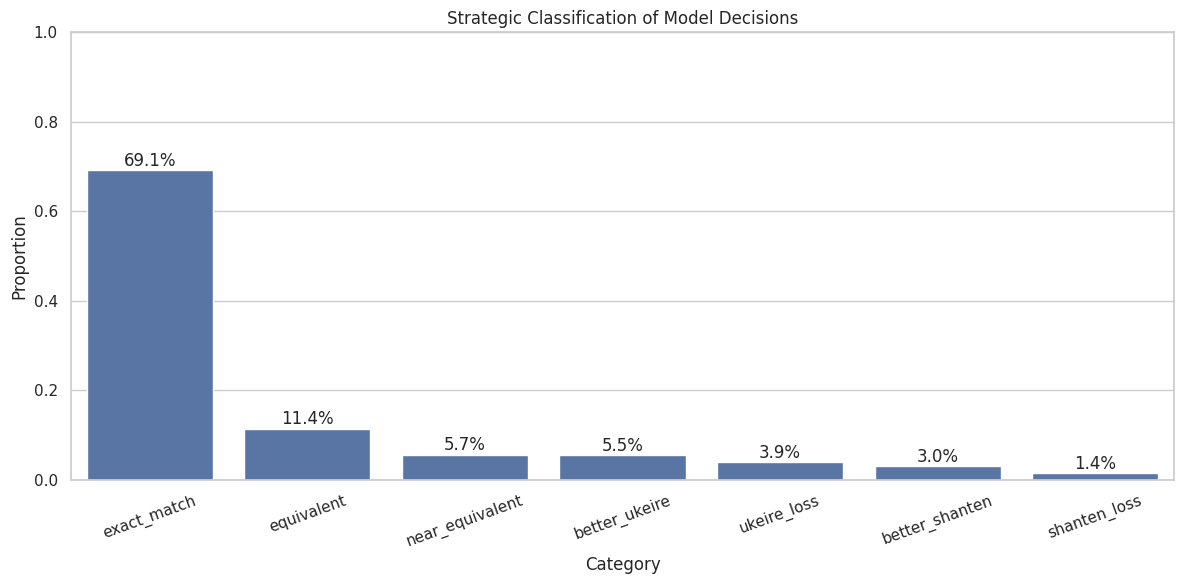
\includegraphics[width=0.8\textwidth]{figures/02_strategic_mistakes.png} 
\caption{Porcentaje de Cada Categoría Estratégica en el Segundo Modelo}
\label{fig:strategic_class_model2}
\end{figure}

Calculando nuevamente el \textit{strategic accuracy} acumulando las categorías de \textit{exact\_match, equivalent, better\_ukeire} y \textit{better\_shanten}, obtenemos un valor ajustado de \textbf{94.6\%}. Esto representa una mejora significativa respecto al accuracy crudo, demostrando que el modelo captura mejor la esencia estratégica del juego más allá de la coincidencia exacta:
\begin{figure}[H]
\centering
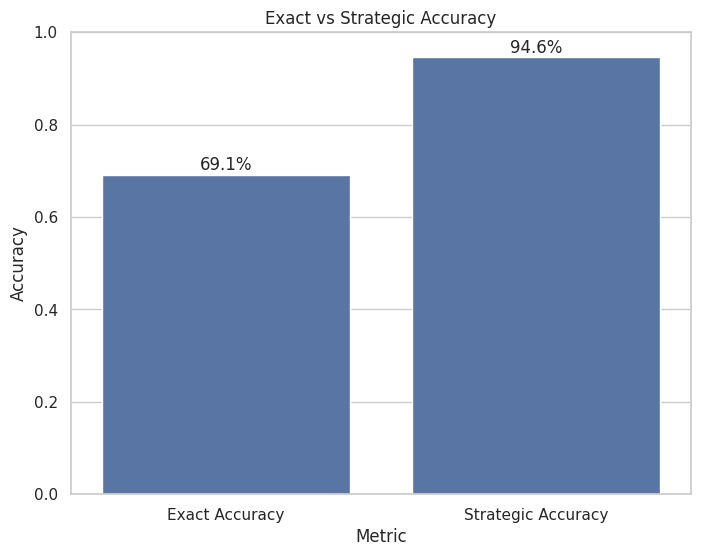
\includegraphics[width=0.8\textwidth]{figures/02_exatvstrategic.png} 
\caption{Comparación validación de accuracy exacta vs accuracy estratégica en el Segundo Modelo}
\label{fig:exact_vs_strat_model2}
\end{figure}

Respecto a la confianza del modelo, la distribución reflejada es bastante similar a la del primer modelo, pero aumenta consideramblemente la confianza en 100\%:
\begin{figure}[H]
\centering
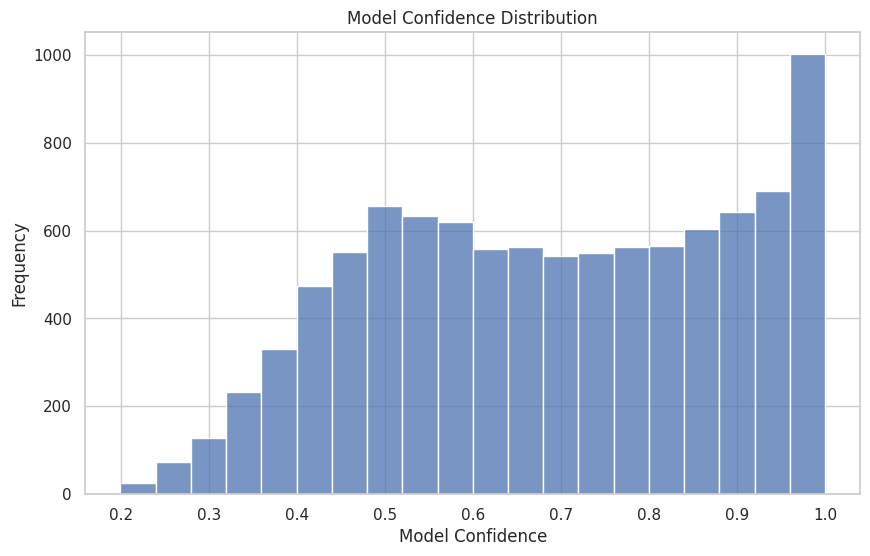
\includegraphics[width=0.8\textwidth]{figures/02_confidence_dist.png} 
\caption{Distribución de confianza del segundo modelo}
\label{fig:confidence_distribution_better_model2}
\end{figure}

Finalmente, podemos ver la descomposición de la confianza por categoría estratégica en este segundo modelo, donde más adelante se realizará una comparación entre los dos modelos:
\begin{figure}[H]
\centering
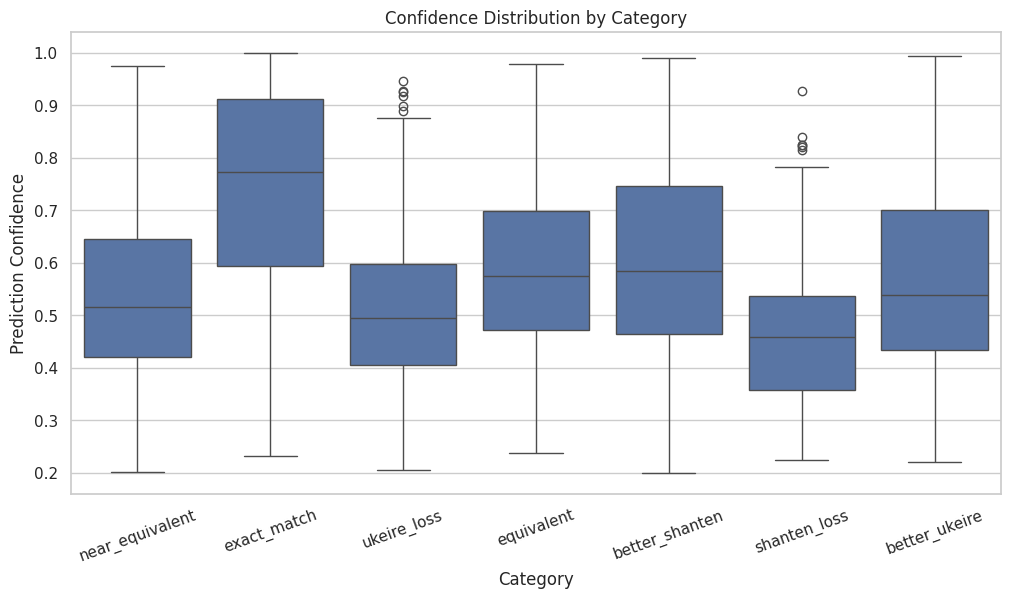
\includegraphics[width=0.8\textwidth]{figures/02_confidence_by_category.png}
\caption{Distribución de confianza del segundo modelo por categoría de la validación estratégica}
\label{fig:confidence_distribution_by_cat_model2}
\end{figure}

\subsubsection{Análisis Comparativo: Impacto del Volumen de Datos}
Para evaluar el impacto directo de la cantidad de datos en el rendimiento estratégico y exacto, se realizó una comparación entre el modelo entrenado con 100k muestras y aquel entrenado con 500k muestras.

En primer lugar, observamos que el aumento del conjunto de entrenamiento generó una mejora significativa en la \textit{exact action accuracy}. El modelo con 500k datos alcanzó un valor de $0.691$, superando al modelo con 100k, cuyo rendimiento se situó en $0.671$. Esta tendencia positiva también se reflejó en la métrica ajustada: el \textit{strategic accuracy} aumentó del $92.4\%$ al $94.6\%$, lo que indica una mayor capacidad del modelo para identificar acciones equivalentes o superiores desde una perspectiva estratégica general:
\begin{figure}[H]
\centering
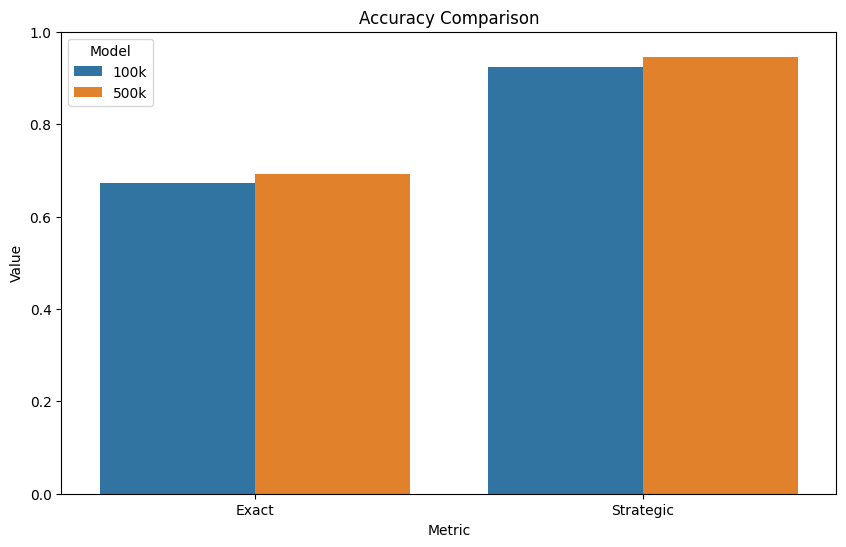
\includegraphics[width=0.8\textwidth]{figures/comparativa_exact_vs_strat.png} 
\caption{Comparación de Accuracy Exacta y Estratégica entre modelos con 100k y 500k de datos}
\label{fig:comp_exact_strat_acc}
\end{figure}

Al analizar la distribución específica por categorías estratégicas, resulta evidente un cambio cualitativo crucial en la toma de decisiones. El modelo entrenado con el conjunto más amplio redujo drásticamente la frecuencia de decisiones que degradan el estado del juego (\textit{shanten-degrading decisions}), pasando de un $3.4\%$ a solo un $1.8\%$. Esta reducción sugiere que el modelo no solo está memorizando respuestas exactas, sino aprendiendo patrones estructurales más profundos que evitan errores estratégicos graves:
\begin{figure}[H]
\centering
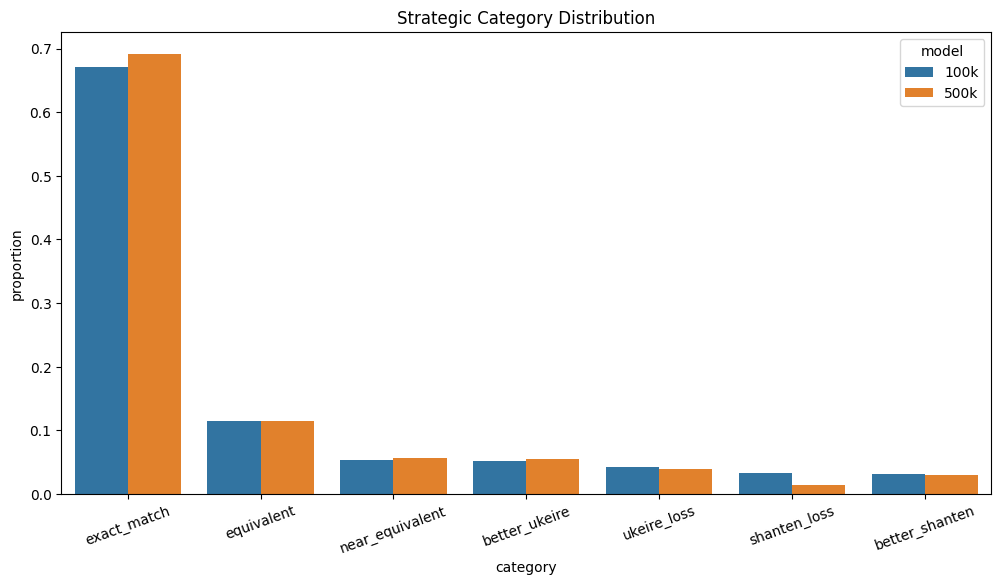
\includegraphics[width=0.8\textwidth]{figures/comparativa_categorias_estrategicas.png}
\caption{Comparación de la distribución de categorías estratégicas entre los dos modelos}
\label{fig:comp_strategic_categories}
\end{figure}

En conclusión, los resultados muestran que el incremento del conjunto de entrenamiento de 100k a 500k muestras produce una mejora consistente en prácticamente todas las métricas evaluadas. El segundo modelo aumenta tanto la \textit{exact accuracy} (67.16\% frente a 69.13\%) como la \textit{strategic accuracy} (92.43\% frente a 94.62\%), además de presentar una mayor confianza media en sus predicciones. Desde el punto de vista estratégico, también se observa una reducción importante de las decisiones que empeoran el Shanten y una mejora del \textit{Mean Ukeire Difference}, que pasa de un valor negativo a uno positivo. Aunque el porcentaje de decisiones clasificadas como \textit{Ukeire Loss} aumenta muy ligeramente (4.3\% frente a 4.4\%), este incremento es prácticamente despreciable y viene acompañado de un mayor número de decisiones \textit{Better Ukeire}, por lo que el balance global continúa siendo claramente favorable para el modelo entrenado con 500k muestras. Estos resultados indican que el aumento del volumen de datos no solo mejora la capacidad del modelo para reproducir decisiones expertas, sino también para realizar descartes estratégicamente más sólidos en una mayor variedad de situaciones de juego.